\documentclass[sigconf,review]{acmart}

\usepackage{booktabs}
\usepackage{tabularx}
\usepackage{array}
\usepackage{microtype}
\usepackage{xcolor}
\usepackage{graphicx}
\usepackage{placeins}

% Give narrow ACM columns enough flexibility to avoid isolated short overfull
% lines without shrinking the document font or scaling tables.
\setlength{\emergencystretch}{2em}

\newcommand{\benchmarktableformat}{%
  \small
  \setlength{\tabcolsep}{4.5pt}%
  \renewcommand{\arraystretch}{1.08}%
}

\setcopyright{none}
\settopmatter{printacmref=true, printccs=true, printfolios=true, authorsperrow=2}
\renewcommand\footnotetextcopyrightpermission[1]{}
\pagestyle{plain}

\acmConference[KDD '27]{The 33rd ACM SIGKDD Conference on Knowledge Discovery and Data Mining}{August 1--5, 2027}{San Jose, CA, USA}
\acmYear{2027}
\copyrightyear{2027}

\title{FinAuth-Audit: Validity-Aware Benchmarking of Financial Agent Authorization}
% KDD 2027 Datasets and Benchmarks single-blind author metadata.
\author{Ke Wang}
\affiliation{%
  \position{Corresponding author}
  \institution{Georgia Institute of Technology}
  \city{Atlanta}
  \state{Georgia}
  \country{United States}
}
\email{colinwang@gatech.edu}

\author{Xiaorui Tang}
\affiliation{%
  \institution{The Hong Kong University of Science and Technology}
  \city{Hong Kong SAR}
  \country{China}
}
\email{alicetang0618@gmail.com}

% Generated by finauth_audit/paper/generate_tables.py. Do not edit manually.
\newcommand{\RealAgentRankSupportStatus}{not supported}
\newcommand{\RealAgentRankSupportClaim}{The preregistered zero-shot inverse rank-transfer criterion is not supported; the independent unit is one UTC date ($n=200$).}
\newcommand{\RealAgentRankIndependentUnit}{UTC date}
\newcommand{\RealAgentRankIndependentUnitCount}{200}
\newcommand{\RealAgentProposalRows}{1,200}
\newcommand{\RealAgentRankSpearman}{0.657}
\newcommand{\RealAgentRankKendall}{0.600}
\newcommand{\RealAgentRankExactP}{0.932}
\newcommand{\RealAgentRankBootstrapMedian}{0.543}
\newcommand{\RealAgentRankBootstrapLCB}{-0.657}
\newcommand{\RealAgentRankBootstrapUCB}{0.943}
\newcommand{\RealAgentRankNegativeProbability}{0.173}
\newcommand{\RealAgentLifecycleOmitSpearman}{1.000}
\newcommand{\RealAgentPairwiseReversalCount}{3}
\newcommand{\RealAgentPairwiseComparisonCount}{15}


\begin{abstract}
Financial agents turn weak priors into actions, but outcome loss, policy violation, and execution authority are distinct. FinAuth-Audit benchmarks whether comparisons among execution rules remain valid when coverage, provenance, consequence severity, review workload, utility, and point-in-time evidence are audited jointly. We benchmark execution rules, not predictors. The release contains 124,000 controlled, provenance, and mechanistic event clusters, public event and order-book layers, and a preregistered 300-date actual-model partition. Four findings define the benchmark. First, the lowest negative-utility authorization rate (NUAR; the frozen artifact field is retained as legacy \texttt{FAR}) is 0.064 but coexists with ALR 0.245, while lineage-clean rules occupy different coverage, utility, and review frontiers. Second, a clean current role retains 0.172 indirect laundering, and partial lineage signatures leave a nonzero finite-sample information cost. Third, a 200-date actual-model test does not reproduce a 60-date pilot inversion and shows that economic loss, material harm, and authority violation rank operating points differently. Fourth, predeclared validity gates retain a powered mixed Binance result, an underpowered event-market layer, and coverage-collapsed learner comparisons rather than promoting partial evidence. FinAuth-Audit is a release protocol, not a trading strategy or deployment claim.
\end{abstract}

\keywords{financial agents, execution authorization, benchmark validity, provenance auditing, abstention, agent safety}

\begin{CCSXML}
<ccs2012>
<concept>
<concept_id>10010147.10010257</concept_id>
<concept_desc>Computing methodologies~Machine learning</concept_desc>
<concept_significance>500</concept_significance>
</concept>
<concept>
<concept_id>10010405.10010489</concept_id>
<concept_desc>Applied computing~Economics</concept_desc>
<concept_significance>300</concept_significance>
</concept>
</ccs2012>
\end{CCSXML}
\ccsdesc[500]{Computing methodologies~Machine learning}
\ccsdesc[300]{Applied computing~Economics}

\begin{document}
\maketitle

\section{Introduction}

Financial AI systems increasingly turn forecasts, learned signals, policy proposals, and language-model assessments into \emph{weak financial priors}: structured beliefs that may inform an action but do not by themselves confer execution authority. Examples include a language model extracting a directional assessment from an earnings release, a forecast model proposing a position change, or a risk system flagging a credit or liquidity condition. In each case the generator proposes; a separate execution rule decides whether to execute, reduce, route to review, or abstain. Existing financial benchmarks primarily evaluate question answering, forecasting, language understanding, or task completion~\cite{chen2021finqa,xie2023pixiu,xie2024finben,wu2023bloomberggpt,yang2023fingpt}. Agent benchmarks extend evaluation to tool use and multi-step interaction~\cite{liu2023agentbench,zhou2023webarena,qin2023toolllm,mialon2023gaia}, but successful prediction or task completion does not establish that a prior deserves execution authority. We therefore benchmark execution rules and the validity of their evaluation, not predictors.

Figure~\ref{fig:overview} gives the running map of the benchmark. In the paper-test operating points, Cost-Aware authorizes 36.7\% of rows and has the lowest NUAR, 0.064, but ALR 0.245. Hard Role Gate authorizes 75.0\% with ALR zero and leads conservative validation hypervolume, but its NUAR is 0.656. Lifecycle has NUAR 0.147, ALR zero, coverage 0.293, and review rate 0.429. No Action receives NUAR \textit{N/A}, not zero. The benchmark therefore exposes a frontier among negative outcomes, lineage integrity, and usable coverage rather than declaring a universal winner.

The validity argument follows four linked threats: NUAR can fall through coverage collapse; current-role metadata can hide lineage laundering; a controlled ranking can fail to transfer across mechanisms or actual-model proposals; and incomplete power or mechanism coverage can make a positive claim undefined. These threats change the evaluation object, so a reproducible low NUAR is not sufficient evidence of valid authorization.

\begin{figure*}[t]
  \centering
  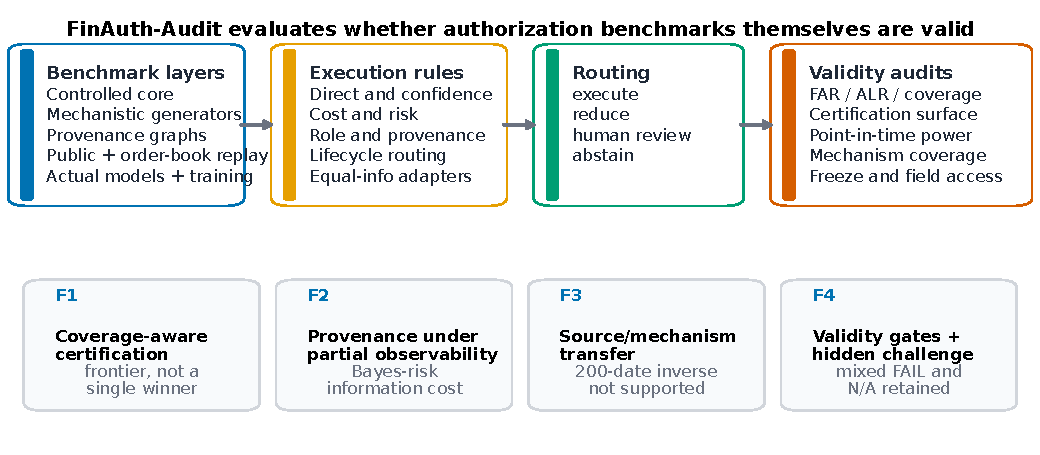
\includegraphics[width=\textwidth]{figures/fig_benchmark_overview.pdf}
  \Description{Flow diagram from benchmark layers through execution rules and four routing decisions to validity audits, followed by four finding boxes for certification, provenance, source transfer, and evidence gates.}
  \caption{\textbf{FinAuth-Audit evaluates whether authorization-benchmark comparisons are valid.} The four stages are benchmark layers, execution rules, routing outcomes, and validity audits. The findings are coverage-aware certification, provenance under partial observability, source and mechanism transfer, and validity gates that retain mixed failures and structural \textit{N/A}.}
  \label{fig:overview}
\end{figure*}

Benchmark outcomes can be fragile to task selection and measurement design~\cite{dehghani2021benchmark,jacobs2021measurement,kiela2021dynabench,ribeiro2020checklist}, while high-stakes data work can accumulate undocumented assumptions and shortcuts~\cite{sambasivan2021data,geirhos2020shortcut,gebru2021datasheets,mitchell2019modelcards}. FinAuth-Audit addresses four coupled blind spots. First, low NUAR can be obtained by suppressing difficult cases. Second, clean current-role metadata can hide upstream lineage laundering. Third, a controlled rule ranking can fail to support its preregistered transfer claim. Fourth, external and training conclusions can be promoted despite insufficient power, collapsed mechanism coverage, or a mixed result.

The benchmark is organized around four linked findings. \textbf{Coverage-aware certification} asks whether NUAR rankings survive joint NUAR, ALR, coverage, utility, and review-load reporting. \textbf{Provenance under partial observability} asks what current roles, full lineage, and missing lineage can identify under delegation, paraphrase, role noise, and multiple hops. \textbf{Transfer validity} asks whether a rule ordering survives mechanism and actual-model shifts. \textbf{Evidence gates} ask whether point-in-time evidence and learned authorization comparisons satisfy predeclared power, effect-size, and mechanism-coverage conditions before positive claims are permitted.

FinAuth-Audit is a benchmark asset and release protocol, not a new execution rule. It contains 124,000 controlled, provenance, and mechanistic event clusters; public event and order-book layers; and a separately frozen 300-date, five-asset, two-task actual-model partition. The latter contains 50 development dates, a one-time 200-date paper test with \RealAgentProposalRows{} cached proposals, and 50 author-unevaluated holdout dates whose proposal plaintext remains encrypted. Latent opportunity, source reliability, costs, stress, and provenance are sampled before rule outputs. Before outcome inspection, existing test clusters were split deterministically into one-time paper tests and community-hidden challenges; evaluators, rules, thresholds, data hashes, and protocols were bound to content-addressed archives.

Our contributions are:
\begin{itemize}
  \item a validity-aware benchmark for execution rules across weak financial priors, with joint coverage, NUAR (legacy artifact field \texttt{FAR}), ALR, utility, missed-opportunity, and review-workload reporting;
  \item branch-neutral utility, sequential-market, and institutional-workflow generators with cluster splits, mechanism holdouts, and a one-time frozen paper/community protocol;
  \item a provenance task with a finite-sample observability limit, direct and indirect laundering, traceable and untraceable delegation, safe-delegation coverage, and structural \textit{N/A}; and
  \item pre-result power, effect-size, and mechanism-coverage gates plus a content-addressed artifact that retains a mixed order-book failure and a larger prospective actual-model test that does not reproduce the inverse rank-transfer pattern observed in a 60-date pilot.
\end{itemize}

EPV serves as one equal-information baseline; removing it does not change any headline conclusion. FinAuth-Audit does not claim deployment readiness, trading profitability, investment advice, public transfer, or a globally optimal rule.

\section{Related Work}

\textbf{Financial and agent benchmarks.} Financial benchmarks evaluate numerical reasoning, language understanding, forecasting, and decision support~\cite{chen2021finqa,xie2023pixiu,xie2024finben,wu2023bloomberggpt,liu2021finrl}. General agent benchmarks evaluate task completion, browsing, and tool use~\cite{liu2023agentbench,zhou2023webarena,qin2023toolllm,mialon2023gaia,yao2023react}. These resources establish important capability measurements, but their evaluation unit is generally a prediction, answer, or completed trajectory rather than the validity of an execution-authority benchmark. Supplementary Table~\ref{tab:benchmark_comparison} locates FinAuth-Audit along that distinction.

\textbf{Selective decisions and safe evaluation.} Selective classification studies prediction with abstention~\cite{elyaniv2010foundations,geifman2017selective}; conformal methods provide distribution-free uncertainty statements under stated assumptions~\cite{vovk2005algorithmic,shafer2008tutorial,angelopoulos2021gentle}; off-policy evaluation estimates policy value from logged behavior~\cite{dudik2011doubly,jiang2016doubly,thomas2016data}; and safe reinforcement learning studies constrained sequential decisions~\cite{garcia2015comprehensive,tamar2015policy}. FinAuth-Audit does not replace these methods. It audits whether a benchmark can distinguish genuine authorization quality from zero coverage, authority leakage, and invalid transfer.

\textbf{Benchmark and model-risk validity.} Benchmark fragility, behavioral testing, measurement validity, data documentation, and shortcut learning motivate stronger evaluation contracts~\cite{dehghani2021benchmark,kiela2021dynabench,ribeiro2020checklist,jacobs2021measurement,gebru2021datasheets,sambasivan2021data,geirhos2020shortcut}. Financial model-risk guidance likewise emphasizes validation, controls, and traceable reporting~\cite{board2011sr117,bis2013principles}. The closest decision-rule perspective evaluates choices across many weak experiments~\cite{chou2025weakrules,bibaut2024covariance,tripuraneni2024choosing}. FinAuth-Audit changes the unit from business experiments to weak financial priors and adds execution coverage, source provenance, point-in-time transfer, and mechanism-level training validity.

\section{Task and Validity Threats}

\subsection{Authorization object}
Each row contains a weak financial prior $p_i$ attached to an event cluster $c(i)$ and a decision-time information set $\mathcal{I}_{t_i}$. Prior generators may be heuristics, forecast models, learned policies, language-model agents, or evidence-only risk systems. The prior specifies a candidate direction, confidence, expected edge, uncertainty, horizon, source identity, and source role. An execution rule $g$ maps only legal fields in $(p_i,\mathcal{I}_{t_i})$ to one of four routes:
\[
  d_i=g(p_i,\mathcal{I}_{t_i})\in\{\texttt{execute},\texttt{reduce},\texttt{review},\texttt{abstain}\}.
\]
Execute and reduce are authorized actions. Review is a deferred workflow and is not execution coverage. Realized return, post-cost utility, harm, tail loss, lineage truth, and future decoys are evaluation fields and are prohibited from deployable rules.

Let $A_i$ indicate an authorized action, $U_i$ denote selected post-cost utility, $H_i=\mathbb{1}[A_i=1\land U_i<0]$, and $L_i$ indicate that an authorized action originated from an ineligible source. For an evaluation profile $S$,
\[
 \mathrm{Cov}(S)=\frac{\sum_{i\in S}A_i}{|S|},\quad
 \mathrm{FAR}(S)=\frac{\sum_{i\in S}H_i}{\sum_{i\in S}A_i},\quad
 \mathrm{ALR}(S)=\frac{\sum_{i\in S}L_i}{\sum_{i\in S}A_i}.
\]
FAR and ALR are \textit{N/A} when $\sum A_i=0$. We define review load as
\[
 \mathrm{Rev}(S)=\frac{1}{|S|}\sum_{i\in S}\mathbb{1}[d_i=\texttt{review}].
\]
Cumulative authorized utility (CAU) sums $U_i$ over authorized rows; missed opportunity cost (MOC) sums the best positive eligible utility on non-authorized rows. Safe-delegation coverage measures authorization of eligible delegated positive opportunities. These quantities describe different objectives and are not collapsed into a scalar leaderboard.

\textbf{Reader map.} Coverage measures how often a rule executes or reduces. FAR measures harmful outcomes conditional on authorization; ALR measures ineligible authority lineage on the same denominator. Review load counts cases deferred to a person. CAU and MOC track authorized and missed positive utility. Structural \textit{N/A} means that a denominator does not exist, not that risk is zero.

For the multi-task actual-model layer, FAR is retained only as a legacy alias for \emph{directional economic-loss authorization}, $\Pr(U<0\mid A=1)$. We separately report material harm, defined by task-specific predeclared severity thresholds; directional tail harm; and authority violation, defined as authorization of an evidence-only risk critic. A losing action is therefore not automatically a material or authority failure, and a profitable action cannot legalize an ineligible source. Structural \textit{N/A} also applies when no development candidate satisfies a preregistered operating-point constraint.

\paragraph{Observable-provenance limit.}
Let $L\in\{0,1\}$ denote laundering truth and let $X$ be any legal observable signature available to a provenance rule. A standard Bayes-classification identity~\cite{devroye1996probabilistic} gives
\begin{equation}
  \inf_h \Pr[h(X)\neq L]
  =\sum_x\min\{\Pr(X=x,L=0),\Pr(X=x,L=1)\}.
  \label{eq:provenance-bayes-risk}
\end{equation}
Under equal class priors this is $(1-\mathrm{TV}(P_{X\mid L=0},P_{X\mid L=1}))/2$. Thus identical legal signatures with conflicting lineage truth impose unavoidable error on every rule measurable with respect to $X$; randomization cannot improve the Bayes risk. FinAuth-Audit reports the plug-in finite-sample value and its exact overlap identity, not a claim that deployed lineage distributions are known. The proof is in the supplement.

\subsection{Four validity threats}
\textbf{Coverage collapse} occurs when a rule suppresses difficult profiles, leaving an apparently low FAR over a narrow authorized subset. \textbf{Provenance laundering} occurs when the current source appears eligible although authority originated from an ineligible source and propagated through delegation, paraphrase, or multiple hops. Full lineage, partial signatures, and current-role-only observations define different identifiability regimes. \textbf{Invalid transfer or training evidence} occurs when public replay violates point-in-time availability, treats derived rows as independent, lacks event-cluster power, or compares learners after mechanism-specific coverage collapses. FinAuth-Audit treats these as benchmark-validity failures, not merely model errors.

\section{Benchmark Construction}

\subsection{Pipeline and data layers}
Supplementary Figure~\ref{fig:overview} summarizes the artifact. Each of 50,000 utility-IID clusters contains four source-role variants, producing 200,000 rows split by cluster into 120,000 training, 40,000 validation, and 40,000 test rows. Before outcome inspection, the 10,000 test clusters were ordered by a SHA-256 rule and split exactly into 5,000 paper-test and 5,000 community-hidden clusters. The seven frozen opportunity slices include ordinary, moderate stress, severe stress, rare safe opportunity, high missed opportunity, stress-only period, and a no-opportunity control.

\paragraph{Branch-neutral construction.} The generator follows a fixed sequence:
\begin{enumerate}
  \item sample an event state, opportunity intent, stress severity, liquidity, and cost regime;
  \item sample four source-role-specific noisy priors and confidence/uncertainty fields;
  \item realize return, full/reduced post-cost utility, and outcome-only harm labels;
  \item attach provenance transformations or task-specific workflow state; and
  \item run execution rules only after the row and legal-field manifest are frozen.
\end{enumerate}
An oracle-positive opportunity indicates that at least one role- and provenance-eligible full or reduced action has positive post-cost utility. It is never a deployable feature. Generator parameters, expected opportunity rates, mechanism holdouts, and seeds are frozen before evaluation; validation defects remain in the negative-results log and were repaired only by rule-independent corrections.

To test generator dependence, we prospectively add two mechanisms without changing rule thresholds: a sequential-market generator with regimes, inventory, market impact, and path dependence, and an institutional-workflow generator with trading, credit, and research-to-action tasks, risk budgets, compliance flags, approval depth, and review pressure. Together they add 96,000 rows from 24,000 clusters. They are mechanistically distinct but still author-controlled scenarios, not market simulators or institutional logs.

\subsection{Provenance layer}
The provenance layer reuses the controlled market-state scaffold but adds role claims, verified roles, original source identifiers, delegation parents, transformation chains, content hashes, hop depth, traceability, and lineage attestation. Five attack families are balanced at the cluster level: clean, role noise, delegation, paraphrase, and multi-hop. Role noise rates are 0\%, 5\%, 10\%, 20\%, and 40\%; hop depths range from one to five. Traceable rows expose enough lineage for detection in principle. Untraceable rows intentionally omit that evidence and are reported as a separate stress/impossibility stratum.

\subsection{Point-in-time public, order-book, and training layers}
The public layer contains 2,500 structurally valid Polymarket event clusters, split chronologically into 1,500 training, 500 validation, and 500 sealed test clusters. The source probability is the last observation strictly before a fixed decision timestamp at 35\% of scheduled lifecycle. Outcome and post-decision fields are labels only. Twenty-three high-activity months reached the frozen pagination cap and are disclosed as truncated. The pre-result power gate estimates 0.164 power, with LCB95 0.160, against a 0.80 requirement, so the layer remains \texttt{exploratory\_only}. FRED and GDELT remain documented extensions rather than confirmatory sources.

A v0.3 extension adds observed market-outcome replay with constructed priors and roles: 185,592 Binance rows from 703 UTC dates and 16,776 licensed MES rows from 233 RTH sessions. Binance combines official banded depth with one-minute BTCUSDT/ETHUSDT bars, split 120/500/83 into development, confirmatory paper test, and hidden dates; planning power uses the frozen v0.2 variance model. MES uses one-contract BBO replay split 60/140/33, with the paper test descriptive only. Both sources reuse frozen priors, rules, and thresholds; outcomes remain sealed until one-time evaluation, and MES rows are not redistributed.

A v0.6 actual-proposal extension uses 300 non-overlapping dates from May 2025 through March 2026, deterministically assigned across BTC, ETH, BNB, SOL, and XRP. Each date contains a directional-execution task with an eligible edge proposer and a 25\% risk-limit-increase task whose source role is deterministically assigned as eligible proposer or evidence-only critic before generation. Three model configurations receive the same legal pre-decision context. The chronological split contains 50 development, 200 one-time paper-test, and 50 author-unevaluated holdout dates. Holdout proposals were generated and encrypted before outcome evaluation; their key remains outside the repository and the ciphertext was not decrypted. Outputs retain malformed placeholders without repair or favorable reruns. Rationales are audit metadata and are excluded from every rule.

The registered training layer freezes D0--D7 at 400 clusters per seed and five seeds. A primary endpoint is valid only when every held-out mechanism has a 95\% coverage lower bound of at least 0.05. A prospective v0.3 robustness study preserves that primary and adds Logistic Regression, histogram gradient boosting, MLP, and selective Logistic learners; 400, 1,000, 5,000, and 20,000-cluster budgets; three curricula; and six held-out mechanisms. The validity condition is deliberately allowed to make a comparison undefined.

\begin{table*}[t]
  \caption{\textbf{FinAuth-Audit releases multiple validity layers rather than a single aggregate row count.} Counts and boundaries are generated from manifests. Controlled, provenance, external order-book, and actual-model results use separately frozen one-time paper tests; the event-market and mechanistic/training extensions retain their stated validation-only or sealed status.}
  \label{tab:dataset_summary}
  \centering
  \benchmarktableformat
  % Generated by finauth_audit/paper/generate_tables.py. Do not edit manually.
\begin{tabular}{p{0.17\linewidth}>{\raggedleft\arraybackslash}p{0.10\linewidth}>{\raggedleft\arraybackslash}p{0.10\linewidth}p{0.23\linewidth}p{0.28\linewidth}}
\toprule
Layer & Rows & Clusters & Split or budget & Coverage / boundary \\
\midrule
Controlled core & 200,000 & 50,000 & 30k / 10k / 5k / 5k clusters & train / val. / paper / hidden \\
Provenance laundering & 200,000 & 50,000 & 30k / 10k / 5k / 5k clusters & 5 attacks; 2 trace strata \\
Mechanistic generators & 96,000 & 24,000 & sequential / institutional & validation robustness; test sealed \\
Public point-in-time & 2,500 & 2,500 & 1.5k / 0.5k / 0.5k & 500 validation reported; test sealed \\
External order book & 202,368 & 936 & Binance 120/500/83; MES 60/140/33 & powered public + licensed descriptive \\
Actual model proposals & 1,200 & 200 & 50 / 200 / 50 dates & 3 models; 2 tasks/date; aggregate only \\
Training utility & 144 fits & 400--20k / curriculum & 3 curricula; 4 learners & 6 mechanisms; N/A retained \\
\bottomrule
\end{tabular}

\end{table*}

\section{Evaluation Protocol}

\subsection{Rules and legal information}
The controlled audit compares No Action, Direct Prior, confidence and uncertainty gates, a risk filter, a cost-aware gate, a hard current-role gate, and a lifecycle checklist. The provenance audit adds No Role Gate, Shared Threshold, Soft Penalty, Provenance Hard Gate, Provenance Learned Gate, and an equal-information EPV Adapter. Equal-information means that the adapter receives the same legal decision-time fields as comparable rules, without outcomes or privileged source evidence. It represents one learned utility-aware rule family and tests whether low NUAR transfers to provenance integrity; it receives no privileged status. The prospective learner suite adds Logistic Regression, histogram gradient boosting, MLP, and a selective Logistic whose threshold is chosen by a frozen coverage-constrained validation rule~\cite{elyaniv2010foundations,geifman2017selective}. These baselines represent distinct authorization designs, and none defines the benchmark identity. Each implementation declares its legal fields, and the feature-access audit fails if a deployable rule uses realized return, utility, negative-outcome labels, laundering truth, tail loss, future decoys, or public outcomes.

\subsection{Cluster-aware bounds and certification}
All uncertainty resamples event clusters, not derived prior rows~\cite{cameron2008bootstrap}. Main controlled and provenance results use 5,000 bootstrap replicates. For each rule and profile, FinAuth-Audit estimates a one-sided 95\% coverage lower bound and NUAR/ALR upper bounds. The frozen certification grid uses
\[
\begin{aligned}
\tau_h&\in\{.05,.10,.15,.20,.25,.30\},\\
\tau_a&\in\{0,.01,.02,.05\},\\
c_{\min}&\in\{.05,.10,.20,.30,.50\}.
\end{aligned}
\]
A cell passes only if
\[
 \begin{aligned}
 \mathrm{UCB}_{.95}(\mathrm{NUAR})&\le\tau_h, &
 \mathrm{UCB}_{.95}(\mathrm{ALR})&\le\tau_a,\\
 \mathrm{LCB}_{.95}(\mathrm{Cov})&\ge c_{\min}.
 \end{aligned}
\]
Certification volume is the passed fraction of the 120 deterministic cells, not a multiple-testing result or weighted leaderboard score. We report the minimum of overall and stress-profile volumes. Coverage collapse is $1-\mathrm{Cov}_{stress}/\mathrm{Cov}_{ordinary}$ and remains undefined when ordinary coverage is zero.

Because the discrete grid encodes risk preferences, we also report five frozen profile grids, a continuous conservative hypervolume, and the NUAR/ALR/coverage/MOC Pareto set on validation. These diagnostics do not select a universal winner. Review is reported separately because routing a case to a person consumes capacity: the artifact evaluates fixed 5\%, 10\%, 20\%, and 40\% review-capacity scenarios and normalized 0.5--5 basis-point review-cost sensitivities.

\subsection{Pre-result gates}
Public evaluation is permitted to become confirmatory only if point-in-time checks, independent-cluster counts, rule coverage, and the frozen power threshold all pass. The gate uses validation uncertainty and structural test-cluster counts without evaluating public test outcomes. Training utility uses a mechanism-wise NUAR endpoint at a validation-fixed target coverage. The endpoint is defined only when every held-out mechanism passes its coverage-LCB floor. D2--D7 are compared with D1 using Holm correction~\cite{holm1979simple}; D0 and the role-neutral control are outside that family. Undefined seed pairs remain absent rather than being imputed as wins or losses.

The v0.6 zero-shot transfer test compares six shared directional rules using economic-loss authorization. Support for the preregistered inverse hypothesis requires both date-bootstrap $\Pr(\rho<0)\ge .95$ and an exact one-sided inverse-or-more-extreme permutation $p\le .05$. Registered diagnostics include Kendall $\tau_b$, leave-one-rule-out, pairwise reversals, and model, asset, and volatility strata; subgroup estimates are not powered confirmatory tests. A secondary in-domain track selects unchanged rule forms from fixed grids using five chronological folds over 50 development dates and a 0.10 execute-or-reduce coverage floor. Selections are frozen before paper outcomes; invalid selections remain \textit{N/A}.

\subsection{One-time paper test and hidden challenge}
After all rules, thresholds, metrics, generators, robustness profiles, and reporting templates were fixed, a deterministic SHA-256 ordering split the 10,000 controlled/provenance test clusters into 5,000 paper-test and 5,000 community-hidden clusters using identifiers only. A validation rehearsal reproduced registered point metrics to within $1.1\times10^{-15}$. The evaluator and scientific surface were then stored in a content-addressed archive with SHA-256 \texttt{be95f4d1...98aa8}; a one-time registry records command, environment, inputs, outputs, and inspection time. The community-hidden, public-test, and FinAuth-Worlds hidden outcomes remain unevaluated. Strict verification checks 475 conditions, including surface hashes and the no-community-access flag.

\section{Benchmark Findings}

\textbf{Evidence tiers.} Headline controlled and provenance results use the one-time 5,000-cluster paper test. Separately frozen tests cover 500 powered Binance dates and 200 dates with \RealAgentProposalRows{} actual-model proposals. MES is descriptive; event-market, cross-generator, and learner analyses are prospective validation evidence. All community-hidden partitions remain unevaluated.

\subsection{Finding 1: Coverage collapse makes low NUAR insufficient}
Table~\ref{tab:main_results} reports the controlled paper test. Direct Prior authorizes every row (NUAR 0.656; ALR 0.250). Cost-Aware has the lowest NUAR, 0.064, but ALR 0.245 and certification volume zero. Lifecycle has NUAR 0.147, ALR zero, certification volume 0.30, coverage 0.293, and review rate 0.429. No Action has zero coverage and NUAR/ALR \textit{N/A}; it cannot win by abstaining everywhere.

The registered stress-to-ordinary coverage audit separates selective omission from uniformly low action rates. Cost-Aware has collapse index \CostAwareCollapseIndex{} and Lifecycle \LifecycleCollapseIndex{}, whereas Direct Prior and Hard Role Gate remain uniform. Thus low NUAR can coexist with materially narrower coverage on difficult profiles.

\begin{table*}[t]
  \caption{\textbf{Paper-test operating points and validation conservative hypervolume reject a single-winner interpretation.} CAU is cumulative authorized utility; MOC is missed opportunity cost; Val. HV is a pre-frozen validation sensitivity. Full certification grids and the Pareto set appear in the supplement. \textit{N/A} denotes structural zero authorization.}
  \label{tab:main_results}
  \centering
  \benchmarktableformat
  % Generated by finauth_audit/paper/generate_tables.py. Do not edit manually.
\begin{tabular}{lrrrrrrr}
\toprule
Rule & Cov. & NUAR & ALR & Review & CAU & MOC & Val. HV \\
\midrule
No Action & 0.000 & \textit{N/A} & \textit{N/A} & 0.000 & 0.00 & 31.20 & 0.000 \\
Direct Prior & 1.000 & 0.656 & 0.250 & 0.000 & 20.38 & 0.00 & 0.000 \\
Confidence Gate & 0.382 & 0.099 & 0.250 & 0.000 & 39.46 & 0.00 & 0.000 \\
Uncertainty Gate & 0.386 & 0.109 & 0.248 & 0.000 & 39.31 & 0.01 & 0.000 \\
Risk Filter & 0.635 & 0.610 & 0.209 & 0.000 & 23.31 & 5.97 & 0.036 \\
Cost-Aware Gate & 0.367 & 0.064 & 0.245 & 0.000 & 40.77 & 0.01 & 0.003 \\
Hard Role Gate & 0.750 & 0.656 & 0.000 & 0.000 & 16.01 & 0.00 & 0.209 \\
Lifecycle Checklist & 0.293 & 0.147 & 0.000 & 0.429 & 30.14 & 0.63 & 0.195 \\
\bottomrule
\end{tabular}

\end{table*}

Validation-to-paper-test rank correlations are effectively 1.000, but frozen policy profiles and continuous hypervolume select different operating points; seven nonzero-action rules lie on the exact four-dimensional Pareto set. \textbf{Finding 1: FinAuth-Audit exposes a multi-objective authorization frontier; low NUAR is neither necessary nor sufficient for a valid comparison.}

\subsection{Finding 2: Clean current roles do not prevent lineage laundering}
Figure~\ref{fig:provenance} and Table~\ref{tab:provenance_results} report the provenance paper test. Hard Role Gate has zero direct leakage but ALR 0.172. Provenance Hard Gate reduces ALR to zero at coverage 0.591 and safe-delegation coverage 0.698; the learned gate raises coverage to 0.603 while accepting ALR 0.018. Low NUAR does not imply clean lineage: Lifecycle has NUAR 0.146 and ALR 0.165; EPV has NUAR 0.039 and ALR 0.169.

\begin{figure*}[t]
  \centering
  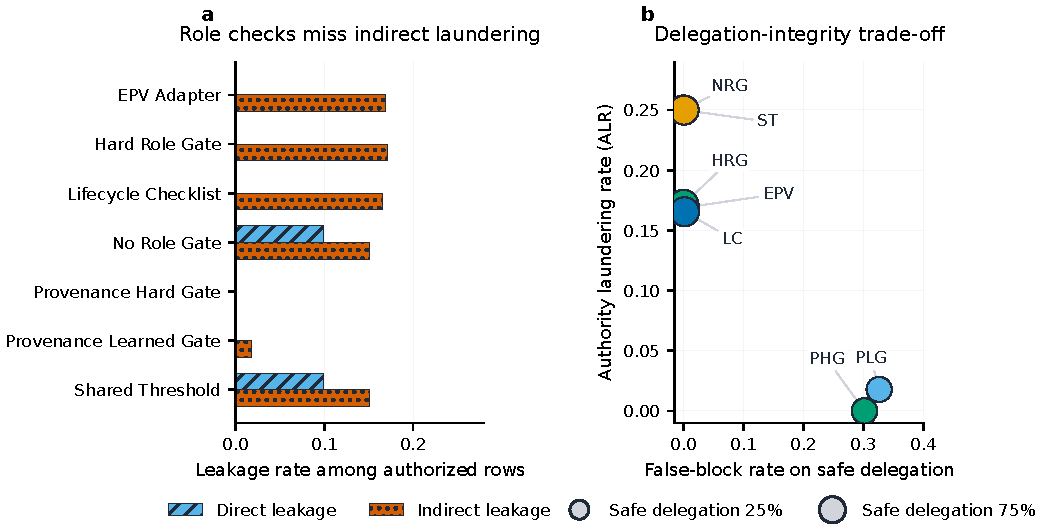
\includegraphics[width=\textwidth]{figures/fig_provenance_laundering.pdf}
  \Description{Two-panel paper-test provenance figure. The left panel compares direct and indirect leakage by rule. The right panel plots authority laundering rate against false-block rate on safe delegation.}
  \caption{\textbf{Current-role integrity, provenance integrity, and usable delegation differ on the paper test.} Panel (a) separates direct from indirect leakage using color and hatch. Panel (b) plots ALR against false blocking; bubble area encodes safe-delegation coverage. Labels abbreviate the rules listed in Table~\ref{tab:provenance_results}.}
  \label{fig:provenance}
\end{figure*}

\begin{table*}[t]
  \caption{\textbf{Paper-test provenance controls trade authorization quality, lineage integrity, delegation coverage, and review load.} Direct and indirect columns are leakage rates among authorized rows.}
  \label{tab:provenance_results}
  \centering
  \benchmarktableformat
  % Generated by finauth_audit/paper/generate_tables.py. Do not edit manually.
\begin{tabular}{lrrrrrrr}
\toprule
Rule & Cov. & FAR & ALR & Direct & Indirect & Safe del. & Review \\
\midrule
No Action & 0.000 & \textit{N/A} & \textit{N/A} & \textit{N/A} & \textit{N/A} & 0.000 & 0.000 \\
No Role Gate & 1.000 & 0.674 & 0.250 & 0.099 & 0.151 & 1.000 & 0.000 \\
Shared Threshold & 0.371 & 0.122 & 0.250 & 0.099 & 0.151 & 0.999 & 0.000 \\
Soft Penalty & 0.406 & 0.198 & 0.238 & 0.085 & 0.153 & 0.999 & 0.000 \\
Hard Role Gate & 0.879 & 0.674 & 0.172 & 0.000 & 0.172 & 1.000 & 0.121 \\
Provenance Hard Gate & 0.591 & 0.674 & 0.000 & 0.000 & 0.000 & 0.698 & 0.183 \\
Provenance Learned Gate & 0.603 & 0.668 & 0.018 & 0.000 & 0.018 & 0.674 & 0.100 \\
Lifecycle Checklist & 0.335 & 0.146 & 0.165 & 0.000 & 0.165 & 0.999 & 0.296 \\
EPV Adapter & 0.297 & 0.039 & 0.169 & 0.000 & 0.169 & 0.999 & 0.000 \\
\bottomrule
\end{tabular}

\end{table*}

The current-role-only Bayes risk is 0.129 on traceable rows and 0.256 on untraceable rows; legal partial signatures reduce it to 0.061 and 0.083. These registered-distribution values quantify ambiguity, not hidden-lineage recovery. \textbf{Finding 2: role eligibility and provenance integrity are distinct targets, and missing lineage creates an identifiable information cost.}

\subsection{Finding 3: The pilot inverse-transfer claim fails to reproduce}
The v0.6 paper test evaluates \RealAgentProposalRows{} cached proposals from three model configurations on two tasks across \RealAgentRankIndependentUnitCount{} independent UTC dates and five assets. The preregistered inverse-rank hypothesis is \RealAgentRankSupportStatus: Spearman $\rho=\RealAgentRankSpearman$, Kendall $\tau_b=\RealAgentRankKendall$, exact one-sided $p=\RealAgentRankExactP$, and bootstrap $\Pr(\rho<0)=\RealAgentRankNegativeProbability$. The binding result therefore retires the 60-date pilot estimate $\rho=-0.928$. Only \RealAgentPairwiseReversalCount{} of \RealAgentPairwiseComparisonCount{} pairs reverse; omitting Lifecycle gives $\rho=\RealAgentLifecycleOmitSpearman$. Nine malformed records remain deterministic non-action placeholders, and subgroup ranks remain diagnostic.

\begin{figure*}[t]
  \centering
  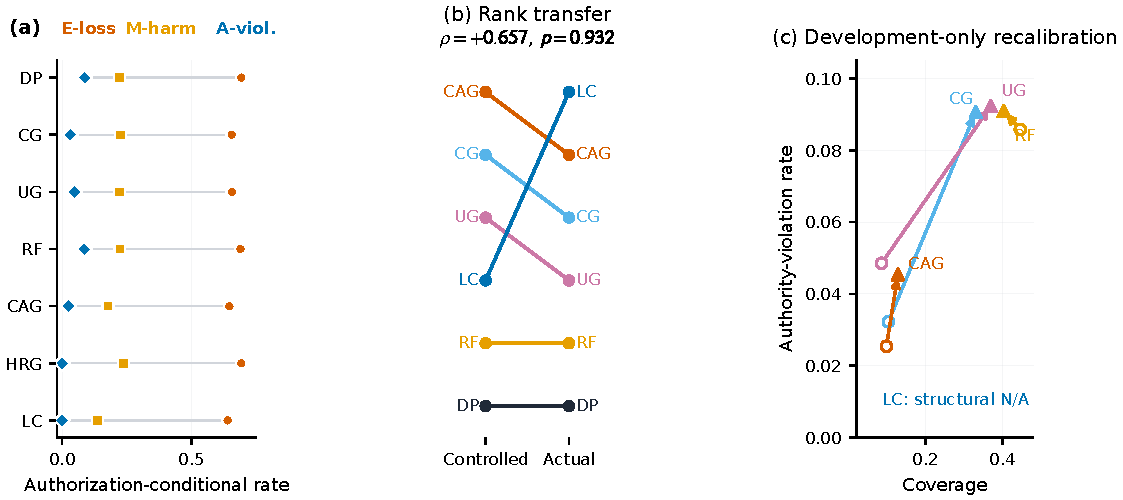
\includegraphics[width=\textwidth]{figures/fig_actual_model_validity.pdf}
  \Description{Three-panel actual-model paper-test figure. Panel a separates economic-loss, material-harm, and authority-violation rates by rule. Panel b compares controlled and actual-model economic-loss ranks. Panel c shows zero-shot to development-recalibrated movement in coverage and authority-violation rate.}
  \caption{\textbf{Actual-model evidence separates consequence semantics, rank transfer, and threshold transport.} Panel (a) distinguishes economic loss, material harm, and authority violation. Panel (b) retains the failed preregistered inverse-rank test. Panel (c) compares zero-shot circles with development-only triangles; Lifecycle is structural \textit{N/A} because no candidate met the coverage floor.}
  \label{fig:actual_model_validity}
\end{figure*}

Endpoint choice changes interpretation: economic loss ranges from 0.641 to 0.694, material harm from 0.138 to 0.238, and authority violation from zero to 0.088. Lifecycle minimizes material harm and authority violation but covers only 0.121. Recalibration raises Confidence and Uncertainty coverage to 0.331 and 0.370 while raising authority violation to 0.091 and 0.092; Lifecycle remains structural \textit{N/A}. Threshold adjustment is not a universal transport repair.

Validation-only mechanistic generators remain less stable against utility IID ($\rho=0.683$ and $0.738$) than against each other ($\rho=0.994$), and the sequential generator certifies no rule. \textbf{Finding 3: the benchmark retires an attractive pilot claim and reports localized sensitivity without replacing a failed primary with subgroups.}

\subsection{Finding 4: Validity gates retain mixed, underpowered, and undefined evidence}
The preregistered 500-date Binance IUT \textbf{fails} despite power 0.970/0.965. Cost-Aware minus Lifecycle passes the negative-utility arm ($-0.0170$, 95\% CI $[-0.0198,-0.0138]$), but laundering rises only $+0.0154$ ($[+0.0140,+0.0168]$), below its $+0.020$ SESOI. MES remains descriptive because its fixed bundle yields a non-estimand role contrast.

The event-market layer passes data-integrity checks but has power 0.164 (LCB95 0.160), below 0.80; it remains \emph{exploratory-only} and sealed.

The registered learner comparison is undefined because a held-out mechanism violates the 5\% coverage-LCB floor. At 20,000 clusters, full-audit and coverage-constrained selective Logistic recover five of six mechanisms, but sequential-market coverage still collapses; complete cross-mechanism NUAR remains \textit{N/A}. \textbf{Finding 4: validity gates retain powered mixed failure, underpowered transfer, and undefined learner evidence instead of converting them into wins.}

Supplementary Figure~\ref{fig:validity_gates} visualizes these unchanged statuses.

\section{Use, Limitations, and Research Opportunities}

\textbf{Community use.} Researchers can implement a rule against the legal-field manifest and run the same certification, provenance, power, and mechanism-coverage checks. The release records routes, hashes, structural \textit{N/A}, and an unevaluated 5,000-cluster community challenge.

\textbf{Scope.} Controlled layers are authorization scenarios, not institutional logs or human labels. Branch-neutral construction and the frozen test support internal validity, but shared generator authorship and legal-field design limit external validity.

\textbf{External limits.} Binance adds observed spread and depth, but constructed priors remain. Actual proposals span five assets and two tasks, while roles remain benchmark-assigned and 200 dates support only aggregate inference. MES is licensed and descriptive; event-market, FRED, and GDELT evidence is non-confirmatory. Review costs are simulated, and the holdout is self-custodied rather than third-party escrow.

\textbf{Research opportunities.} The coverage-constrained learner is a negative anchor, not a winner; the actual-proposal audit likewise retires the pilot inversion and rejects universal threshold repair. Independently authored generators, practitioner-labelled authorization tasks, third-party challenge custody, and stronger point-in-time data are the next external-validity tests. FinAuth-Audit remains an offline benchmark, not investment advice or institutional approval.

\section{Conclusion}
FinAuth-Audit makes validity part of financial-agent authorization evaluation. Low NUAR can coexist with coverage collapse or lineage laundering; controlled ranks need not support a preregistered transfer claim; and weak external or learner evidence must remain exploratory or \textit{N/A}. The \href{https://github.com/colin-wang-research/finanth-audit}{public artifact} preserves each frozen surface and adverse result. It supports reproducible rule comparison without treating ex post loss, prediction quality, a source, a baseline, or one metric as execution authority.


\FloatBarrier
\clearpage
\balance
\bibliographystyle{ACM-Reference-Format}
\bibliography{references}
\nobalance

\clearpage
\appendix
\raggedbottom
\section{Artifact and Reproduction}
The aggregate v0.6 release combines the frozen v0.2 controlled/provenance
surface, prospective robustness extensions, the separately frozen v0.3
external order-book surface, and the frozen v0.6 actual-model proposal
extension. Every data and result layer records a configuration hash, data hash,
split registry, seed registry, output hashes, and claim boundary. The aggregate
verifier transitively checks the earlier surfaces and the v0.6 freeze-to-result
chain; the repository suite is rerun before release. The controlled paper
test is bound to content-addressed archive \texttt{be95f4d1...98aa8} and took
80.59 seconds on the development machine with peak resident memory about
550 MB. Re-running any inspected one-time paper test is prohibited except for a
versioned correctness defect that preserves the original output.

\begin{table*}[h]
  \caption{\textbf{FinAuth-Audit treats benchmark validity as the evaluation object.} ``Rules'' denotes explicit comparison of execution or decision rules; the remaining columns denote validity audits, not generic safety features.}
  \label{tab:benchmark_comparison}
  \centering
  \benchmarktableformat
  % Generated by finauth_audit/paper/generate_tables.py. Do not edit manually.
\begin{tabular}{llcccc}
\toprule
Benchmark & Evaluation unit & Rules & Coverage audit & Provenance & Power gate \\
\midrule
FinQA~\cite{chen2021finqa} & financial QA & no & no & no & no \\
PIXIU~\cite{xie2023pixiu} & financial tasks & no & no & no & no \\
FinBen~\cite{xie2024finben} & financial tasks & no & no & no & no \\
AgentBench~\cite{liu2023agentbench} & agent tasks & no & no & no & no \\
WebArena~\cite{zhou2023webarena} & web tasks & no & no & no & no \\
Weak experiments~\cite{chou2025weakrules} & experiment portfolios & yes & no & no & no \\
\textbf{FinAuth-Audit} & weak financial priors & yes & yes & yes & yes \\
\bottomrule
\end{tabular}

\end{table*}

\begin{table*}[h]
  \caption{Artifact components and machine-checkable release paths.}
  \label{tab:artifact_checklist}
  \centering
  \benchmarktableformat
  % Generated by finauth_audit/paper/generate_tables.py. Do not edit manually.
\begin{tabular}{p{0.20\linewidth}p{0.35\linewidth}p{0.31\linewidth}}
\toprule
Artifact & Release path & Verification \\
\midrule
Paper test & \path{results/paper_test/} & one-time registry; 5k clusters \\
Community hidden & \path{sealed/community_hidden/} & 5k clusters; unevaluated \\
Freeze archive & \path{manifests/paper_test_snapshots/} & content-addressed SHA-256 \\
Point-in-time layer & \path{results/public_audit/} & power and timestamp gates \\
External order book & \path{results/external_orderbook_v03/} & powered mixed result; 550 checks \\
Actual-model paper test & \path{results/real_agent_v06/paper_test/} & 3 models; 200-date, 2-task aggregate test \\
Historical-memory audit & \path{results/real_agent_v06/historical_memory_audit/} & outcome-blind aggregates; no rationale text persisted \\
Training robustness & \path{results/training_robustness_v03/} & 144 fits; 6 mechanisms \\
Figures & \path{paper/figures/} & PDF, SVG, PNG; text QA \\
HTML and cards & \path{paper/html/}; \path{docs/} & combined paper/supplement; local assets \\
Release archive & \path{dist/finauth-audit-0.6.0.tar.gz} & allowlist; clean-room hash and split scan \\
Verifier & \path{verify_artifact.py} & all frozen surfaces, fields, hashes, and tests \\
\bottomrule
\end{tabular}

\end{table*}

The figure generator writes PDF, SVG, and PNG from one source and records a minimum visible font size of 8 pt. Generation fails if marked point labels overlap. The table generator reads frozen result files and records input/output hashes in \texttt{table\_manifest.json}; no reported numeric result is hand-entered into the manuscript. A page-faithful HTML bundle mirrors the combined PDF, while the benchmark card, reproduction guide, maintenance policy, and external-submission protocol state the community-use contract.

\begin{figure*}[h]
  \centering
  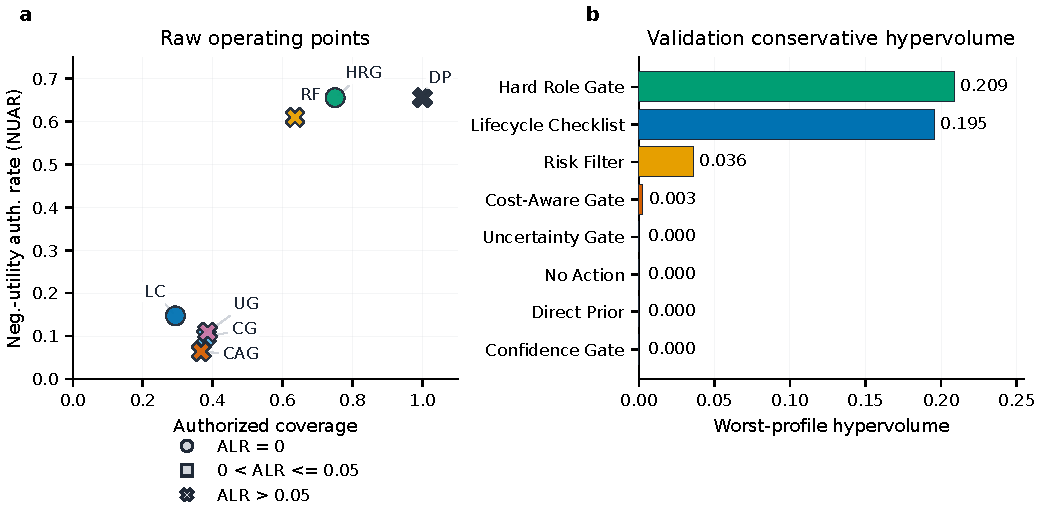
\includegraphics[width=\textwidth]{figures/fig_certification_surface.pdf}
  \Description{Two-panel validity figure. The left panel plots paper-test rule coverage against negative-utility authorization rate with marker shape indicating authority-laundering strata. The right panel ranks validation worst-profile conservative hypervolume.}
  \caption{\textbf{NUAR, lineage integrity, coverage, and conservative hypervolume produce different rule orderings.} Panel (a) reports one-time paper-test operating points; marker shape encodes ALR strata. Short labels are DP (Direct Prior), CG (Confidence Gate), UG (Uncertainty Gate), RF (Risk Filter), CAG (Cost-Aware Gate), HRG (Hard Role Gate), and LC (Lifecycle Checklist). Panel (b) is a pre-frozen validation sensitivity, not a second paper-test ranking. Zero authorization produces NUAR and ALR \textit{N/A}, not zero.}
  \label{fig:certification}
\end{figure*}

\section{Controlled Certification Details}
The controlled evaluation excludes the explicit no-opportunity slice from certification but reports it as a negative control. Table~\ref{tab:certification_profiles} gives the cluster-bootstrap bounds used by the frozen 120-cell surface. A zero-action bootstrap replicate contributes coverage zero and execution-denominator metrics \textit{N/A}. If every replicate is undefined, no dependent cell passes.

\begin{table*}[h]
  \caption{\textbf{Pre-frozen policy families and continuous hypervolume do not define a universal winner.} Values are worst-profile validation pass fractions over each author-specified grid. The conservative family certifies no rule; Lifecycle has nonzero balanced and coverage-first volume, while Hard Role Gate has the largest continuous conservative hypervolume. These are sensitivity diagnostics, not practitioner-elicited thresholds.}
  \label{tab:policy_families}
  \centering
  \benchmarktableformat
  % Generated by finauth_audit/paper/generate_tables.py. Do not edit manually.
\begin{tabular}{lrrrr}
\toprule
Rule & Conservative & Balanced & Coverage-first & Continuous HV \\
\midrule
No Action & 0.000 & 0.000 & 0.000 & 0.000 \\
Direct Prior & 0.000 & 0.000 & 0.000 & 0.000 \\
Confidence Gate & 0.000 & 0.000 & 0.000 & 0.000 \\
Uncertainty Gate & 0.000 & 0.000 & 0.000 & 0.000 \\
Risk Filter & 0.000 & 0.000 & 0.000 & 0.036 \\
Cost-Aware Gate & 0.000 & 0.000 & 0.000 & 0.003 \\
Hard Role Gate & 0.000 & 0.000 & 0.000 & 0.209 \\
Lifecycle Checklist & 0.000 & 0.375 & 0.188 & 0.195 \\
\bottomrule
\end{tabular}

\end{table*}

\begin{table*}[h]
\caption{One-sided cluster-bootstrap bounds and certification volumes by rule and profile on the paper test.}
  \label{tab:certification_profiles}
  \centering
  \benchmarktableformat
  % Generated by finauth_audit/paper/generate_tables.py. Do not edit manually.
\begin{tabular}{llrrrr}
\toprule
Rule & Profile & Coverage LCB & NUAR UCB & ALR UCB & Cert. volume \\
\midrule
No Action & overall & 0.000 & \textit{N/A} & \textit{N/A} & 0.000 \\
No Action & stress & 0.000 & \textit{N/A} & \textit{N/A} & 0.000 \\
Direct Prior & overall & 1.000 & 0.667 & 0.250 & 0.000 \\
Direct Prior & stress & 1.000 & 0.712 & 0.250 & 0.000 \\
Confidence Gate & overall & 0.370 & 0.107 & 0.253 & 0.000 \\
Confidence Gate & stress & 0.341 & 0.161 & 0.254 & 0.000 \\
Uncertainty Gate & overall & 0.375 & 0.117 & 0.250 & 0.000 \\
Uncertainty Gate & stress & 0.346 & 0.174 & 0.250 & 0.000 \\
Risk Filter & overall & 0.625 & 0.624 & 0.211 & 0.000 \\
Risk Filter & stress & 0.469 & 0.678 & 0.177 & 0.000 \\
Cost-Aware Gate & overall & 0.356 & 0.069 & 0.247 & 0.000 \\
Cost-Aware Gate & stress & 0.302 & 0.053 & 0.248 & 0.000 \\
Hard Role Gate & overall & 0.750 & 0.667 & 0.000 & 0.000 \\
Hard Role Gate & stress & 0.750 & 0.713 & 0.000 & 0.000 \\
Lifecycle Checklist & overall & 0.285 & 0.156 & 0.000 & 0.300 \\
Lifecycle Checklist & stress & 0.233 & 0.127 & 0.000 & 0.400 \\
\bottomrule
\end{tabular}

\end{table*}

The paper-test opportunity rates are ordinary 0.450, moderate stress 0.386, severe stress 0.236, rare safe opportunity 0.131, high missed opportunity 0.507, stress-only period 0.195, and no-opportunity control 0.000. The oracle-positive label is outcome-only and is never available to a rule.

\section{Provenance Definitions and Strata}
Direct leakage authorizes a currently ineligible source. Indirect leakage authorizes a currently eligible source whose original authority is ineligible. ALR uses the same authorized-action denominator as indirect laundering truth. Safe-delegation coverage is the fraction of eligible delegated positive opportunities that remain authorized; false block is its complement. Table~\ref{tab:provenance_traceability} separates the traceable and untraceable strata.

\begin{table*}[h]
\caption{Traceability-specific provenance outcomes on the paper test. \textit{N/A} is structural when a rule authorizes zero rows in a stratum.}
  \label{tab:provenance_traceability}
  \centering
  \benchmarktableformat
  % Generated by finauth_audit/paper/generate_tables.py. Do not edit manually.
\begin{tabular}{llrrrl}
\toprule
Rule & Traceability & Cov. & ALR & Safe del. & False block \\
\midrule
EPV Adapter & traceable & 0.288 & 0.148 & 0.999 & 0.001 \\
EPV Adapter & untraceable & 0.338 & 0.248 & 0.998 & 0.002 \\
Hard Role Gate & traceable & 0.851 & 0.150 & 1.000 & 0.000 \\
Hard Role Gate & untraceable & 1.000 & 0.254 & 1.000 & 0.000 \\
Lifecycle Checklist & traceable & 0.325 & 0.145 & 0.999 & 0.001 \\
Lifecycle Checklist & untraceable & 0.378 & 0.244 & 0.998 & 0.002 \\
No Action & traceable & 0.000 & \textit{N/A} & 0.000 & 1.000 \\
No Action & untraceable & 0.000 & \textit{N/A} & 0.000 & 1.000 \\
No Role Gate & traceable & 1.000 & 0.249 & 1.000 & 0.000 \\
No Role Gate & untraceable & 1.000 & 0.254 & 1.000 & 0.000 \\
Provenance Hard Gate & traceable & 0.724 & 0.000 & 1.000 & 0.000 \\
Provenance Hard Gate & untraceable & 0.000 & \textit{N/A} & 0.000 & 1.000 \\
Provenance Learned Gate & traceable & 0.627 & 0.015 & 0.676 & 0.324 \\
Provenance Learned Gate & untraceable & 0.497 & 0.035 & 0.668 & 0.332 \\
Shared Threshold & traceable & 0.370 & 0.249 & 1.000 & 0.000 \\
Shared Threshold & untraceable & 0.376 & 0.252 & 0.999 & 0.001 \\
Soft Penalty & traceable & 0.404 & 0.234 & 1.000 & 0.000 \\
Soft Penalty & untraceable & 0.416 & 0.254 & 0.999 & 0.001 \\
\bottomrule
\end{tabular}

\end{table*}

Traceable rows include the attested lineage-role chain needed to detect laundering in principle. Untraceable rows omit that evidence. On the paper test, Provenance Hard Gate has traceable coverage 0.724 and untraceable coverage zero; its untraceable NUAR and ALR are undefined rather than zero. The empirical current-role-only Bayes error lower bound rises from 0.129 on traceable rows to 0.256 on untraceable rows, while legal partial signatures reduce the corresponding bounds to 0.061 and 0.083. This is an evidence-availability boundary, not a claim that a detector should infer hidden lineage.

\paragraph{Proof of Equation~\eqref{eq:provenance-bayes-risk}.}
For a fixed observable signature $x$, any deterministic rule $h$ predicts either zero or one. Its error mass at $x$ is therefore either $\Pr(X=x,L=1)$ or $\Pr(X=x,L=0)$, and the smaller achievable mass is their minimum. Summing independently over signatures proves the first equality. A randomized rule takes a convex combination of the same two error masses and cannot improve the minimum. Under equal priors, write $p_\ell(x)=\Pr(X=x\mid L=\ell)$; then
\begin{align*}
 \sum_x \min\{\tfrac12p_0(x),\tfrac12p_1(x)\}
 &=\tfrac12\left(1-\tfrac12\sum_x|p_0(x)-p_1(x)|\right)\\
 &=\tfrac12(1-\mathrm{TV}(P_0,P_1)).
\end{align*}
The audit uses empirical signature frequencies in place of joint probabilities. Its minority count is the exact minimum empirical error for rules using that signature, not a distribution-free bound for another institution or period.

\paragraph{Derivation of Equation~\eqref{eq:provenance-partial-id}.}
Write $q(x)=\Pr(L=1\mid X=x)$. For any rule with positive coverage,
$\mathrm{ALR}(a)=\mathbb{E}[a(X)q(X)]/\mathbb{E}[a(X)]$.
Multiplying the pointwise bounds $\ell(x)\le q(x)\le u(x)$ by the
nonnegative weight $a(x)\Pr(X=x)$, summing, and dividing by coverage gives
Equation~\eqref{eq:provenance-partial-id}. Pointwise-compatible choices of
$q(x)$ attain both endpoints. If resolved signatures have $u=\ell$ and
unresolved signatures have $[\ell,u]=[0,1]$, the interval width is exactly
the rule's authorized unresolved mass divided by its total authorized mass.

\begin{table*}[h]
  \caption{\textbf{Legal observability controls the minimum empirical laundering-classification error.} Joint separation is the weighted empirical separation term in Equation~\eqref{eq:provenance-bayes-risk}; the implementation verifies the corresponding overlap identity to numerical precision.}
  \label{tab:provenance_identifiability}
  \centering
  \benchmarktableformat
  % Generated by finauth_audit/paper/generate_tables.py. Do not edit manually.
\begin{tabular}{llrrrr}
\toprule
Traceability & Observable signature & Rows & Collision frac. & Bayes risk & Joint sep. \\
\midrule
traceable & current role only & 32,857 & 1.000 & 0.129 & 0.742 \\
traceable & legal partial signature & 32,857 & 0.720 & 0.061 & 0.877 \\
untraceable & current role only & 7,143 & 1.000 & 0.256 & 0.488 \\
untraceable & legal partial signature & 7,143 & 0.519 & 0.083 & 0.834 \\
\bottomrule
\end{tabular}

\end{table*}

\section{Public Point-in-Time Gate}
The Polymarket metadata window is 2022-01-01 through 2026-07-17. Monthly sampling caps each month at 120 clusters and each series/month at 12 clusters. Twenty-three high-activity months reached the frozen pagination limit and are disclosed as truncated. Historical probability comes from CLOB price history when available and documented public trades otherwise. The fixed decision time is 35\% of scheduled lifecycle; the source probability precedes the decision, and the first execution observation follows it but precedes resolution.

\begin{table*}[h]
  \caption{Public-source classifications and the pre-result power gate. The point-in-time layer remains \texttt{exploratory\_only} because power is below the frozen requirement; no public test outcome is reported.}
  \label{tab:public_power}
  \centering
  \benchmarktableformat
  % Generated by finauth_audit/paper/generate_tables.py. Do not edit manually.
\begin{tabular}{llrrrp{0.29\linewidth}}
\toprule
Layer / source & Clusters & Power & LCB95 & Req. & Classification \\
\midrule
Public point-in-time & 500 (structural) & 0.164 & 0.160 & 0.80 & exploratory\_only \\
polymarket &  &  &  &  & descriptive public-derived \\
polymarket\_repeated &  &  &  &  & excluded from inference \\
gdelt &  &  &  &  & controlled information-shock \\
fred &  &  &  &  & exploratory non-vintage \\
polymarket\_point\_in\_time &  &  &  &  & confirmatory candidate; structural only \\
\bottomrule
\end{tabular}

\end{table*}

The first CLOB-only design produced sufficient histories for 516 candidate markets. A documented read-only trades fallback increased structural usability without creating synthetic probabilities, spread, or depth. An earlier 3,000-cluster design covered only about 19 hours and was rejected as externally narrow before result inspection. Both negative design iterations remain in the project log.

\section{External Order-Book Replication}
The separately versioned v0.3 extension freezes public Binance USD-M futures
banded depth plus one-minute bars and licensed Databento MES BBO before outcome
evaluation. It is observed market-outcome replay with constructed priors and
assigned roles. Binance uses 500 UTC-date paper-test clusters; planning power
under the frozen v0.2 variance model is 0.970 and 0.965 for the two registered
SESOIs. MES uses 140 RTH-session clusters
and is classified as descriptive because its corresponding design powers are
0.528 and 0.514. Feature rows and sealed execution inputs are separate; returns,
post-cost utility, harm, and burden are materialized only after freeze
verification inside the write-once evaluator.

\begin{table*}[h]
  \caption{\textbf{The external intersection-union claim fails, and observed market data do not make weak priors or authority roles observational.} Panel A reports Cost-Aware Gate minus Lifecycle Checklist. Binance is confirmatory; MES is licensed descriptive evidence, and its fixed six-prior laundering contrast is structural. Panel B separates observed, pre-decision derived, benchmark-assigned, and sealed outcome-only fields.}
  \label{tab:external_orderbook}
  \label{tab:external_field_origins}
  \centering
  \benchmarktableformat
  \textit{Panel A: frozen external replication outcomes.}\par\smallskip
  % Generated by finauth_audit/paper/generate_tables.py. Do not edit manually.
\begin{tabular}{llrlrrrp{0.18\linewidth}}
\toprule
Source & Evidence & Clusters & Endpoint & Diff. & 95\% CI & SESOI & Status \\
\midrule
Binance & powered public & 500 & False-auth. burden & -0.017 & [-0.020, -0.014] & $\leq -0.015$ & pass \\
Binance & powered public & 500 & Laundering burden & +0.015 & [+0.014, +0.017] & $\geq +0.020$ & fail \\
Binance & powered public & 500 & Intersection-union & -- & -- & both arms & \textbf{FAIL (1/2)} \\
MES & licensed descriptive & 140 & False-auth. burden & -0.019 & [-0.029, -0.010] & $\leq -0.015$ & descriptive \\
MES & licensed descriptive & 140 & Laundering burden & 1/6 by design & -- & not applied & not an estimand \\
\bottomrule
\end{tabular}

  \par\medskip
  \textit{Panel B: field origins and evaluation boundary.}\par\smallskip
  % Generated by finauth_audit/paper/generate_tables.py. Do not edit manually.
\begin{tabular}{p{0.19\linewidth}p{0.34\linewidth}p{0.39\linewidth}}
\toprule
Origin & Fields & Evaluation boundary \\
\midrule
Observed source & quotes, bars, depth, timestamps & available at or before the registered decision time \\
Pre-decision derived & momentum, volatility, imbalance, spread/cost proxies & deterministic functions of observed source fields \\
Benchmark assigned & prior family, action, confidence, source role, eligibility & frozen weak-prior construction; not observed agent behavior \\
Outcome only & entry/exit prices, return, utility, harm, burden & sealed until the one-time evaluator; illegal for deployable rules \\
\bottomrule
\end{tabular}

  \par\medskip
  \begin{minipage}{0.96\textwidth}
  \small
  \textit{Sensitivity and release boundary.}
  The Binance seven-day moving-block sensitivity preserves the arm-level
  interpretation. At the frozen primary 8-bps fee, only the registered
  \texttt{false\_authorization\_burden} endpoint (negative-utility burden)
  passes. A 4-bps sensitivity passes both arms, whereas 12 bps passes
  neither; these fee-grid results use fewer bootstrap replicates and remain
  secondary. No sensitivity replaces the registered primary. Binance releases
  source archives, official checksums, derived rows, manifests, and code. MES
  reproduction requires Databento entitlement, and row-level licensed data are
  not redistributed. MES is an optional licensed replication layer; all
  headline benchmark functionality and primary controlled/provenance
  evaluations are reproducible without redistributing MES records. The public
  dataset entry, exact schema, date/session definitions, reconstruction scripts,
  manifests, and checksums are documented in the artifact.
  \end{minipage}
\end{table*}

\FloatBarrier

\section{Actual Model Proposal Extension}
The v0.6 extension evaluates actual cached proposal outputs rather than
deterministic agent stubs. GPT-5.4-mini, GPT-5.5, and Claude Sonnet 4.6 receive
the same legal pre-decision context on 300 independent dates assigned across
BTC, ETH, BNB, SOL, and XRP. Each date includes a directional-execution task and
a 25\% risk-limit-increase task. Directional sources are eligible edge
proposers; risk-limit source role is assigned by frozen event-ID parity as an
eligible proposer or evidence-only critic before generation. The chronological
partition is 50 development, 200 one-time paper test, and 50 author-unevaluated
holdout dates. The holdout contexts were sent to the same model configurations
before outcome evaluation; 300 proposal rows were encrypted, their key remains
outside the repository, and the ciphertext was not decrypted.

The development/paper cache contains 1,500 plaintext proposal rows and has raw
schema validity 0.994. Nine expected records remain malformed placeholders,
there are zero repairs, and no outcome-conditioned or favorable rerun is
permitted. One extra record was ignored under the preapproved duplicate/extra
record policy. Rationales and self-reported evidence are retained in private
audit caches but prohibited from every execution rule and excluded from the
aggregate public release. The explicit historical-memory lexical audit finds no
registered retrospective phrase, but cannot establish absence of implicit
model memory.

\begin{table*}[h]
  \caption{\textbf{Economic loss, material harm, and authority violation are distinct zero-shot endpoints.} The table reports overall operating points across \RealAgentRankIndependentUnitCount{} UTC-date clusters. Economic loss applies to directional authorization; material harm pools preregistered task-specific severity; authority violation enforces the declared evidence-only critic boundary. Utility is normalized task utility, not profit.}
  \label{tab:real_agent_overall}
  \centering
  \benchmarktableformat
  % Generated by finauth_audit/paper/generate_tables.py. Do not edit manually.
\begin{tabular}{lrrrrrrrr}
\toprule
Rule & Dates & Cov. & Econ. loss & Material harm & Tail harm & Authority viol. & Utility & Review \\
\midrule
Direct Prior & 200 & 0.457 & 0.694 & 0.223 & 0.078 & 0.088 & -0.155 & 0.000 \\
Confidence Gate & 200 & 0.103 & 0.657 & 0.226 & 0.088 & 0.032 & -0.029 & 0.000 \\
Uncertainty Gate & 200 & 0.086 & 0.658 & 0.223 & 0.053 & 0.049 & -0.021 & 0.000 \\
Risk Filter & 200 & 0.447 & 0.690 & 0.224 & 0.079 & 0.086 & -0.154 & 0.000 \\
Cost-Aware Gate & 200 & 0.098 & 0.648 & 0.178 & 0.019 & 0.025 & -0.023 & 0.000 \\
Hard Role Gate & 200 & 0.417 & 0.694 & 0.238 & 0.078 & 0.000 & -0.144 & 0.000 \\
Lifecycle Checklist & 200 & 0.121 & 0.641 & 0.138 & 0.015 & 0.000 & -0.025 & 0.069 \\
\bottomrule
\end{tabular}

\end{table*}

\begin{table*}[h]
  \caption{\textbf{Task-specific zero-shot and development-recalibrated operating points retain structural \textit{N/A}.} Bounds use 10,000 UTC-date cluster-bootstrap replicates over 200 dates. Model abstention remains in the task denominator but cannot be authorized. Lifecycle has no recalibrated point because no development candidate meets the frozen coverage floor.}
  \label{tab:real_agent_rules}
  \centering
  \benchmarktableformat
  % Generated by finauth_audit/paper/generate_tables.py. Do not edit manually.
\begin{tabular}{lllrrrr}
\toprule
Track & Task & Rule & Cov. [95\%] & Task harm [95\%] & Authority viol. & Utility \\
\midrule
Zero-shot & Directional & Direct Prior & 0.642 [0.590, 0.692] & 0.694 [0.620, 0.765] & 0.000 & -0.262 \\
Zero-shot & Directional & Confidence Gate & 0.170 [0.135, 0.205] & 0.657 [0.537, 0.769] & 0.000 & -0.053 \\
Zero-shot & Directional & Uncertainty Gate & 0.127 [0.097, 0.158] & 0.658 [0.521, 0.787] & 0.000 & -0.037 \\
Zero-shot & Directional & Risk Filter & 0.630 [0.577, 0.682] & 0.690 [0.615, 0.764] & 0.000 & -0.260 \\
Zero-shot & Directional & Cost-Aware Gate & 0.175 [0.137, 0.215] & 0.648 [0.515, 0.770] & 0.000 & -0.044 \\
Zero-shot & Directional & Hard Role Gate & 0.642 [0.590, 0.693] & 0.694 [0.618, 0.767] & 0.000 & -0.262 \\
Zero-shot & Directional & Lifecycle Checklist & 0.218 [0.173, 0.265] & 0.641 [0.517, 0.760] & 0.000 & -0.047 \\
Zero-shot & Risk-limit & Direct Prior & 0.272 [0.227, 0.318] & 0.074 [0.021, 0.138] & 0.294 & -0.048 \\
Zero-shot & Risk-limit & Confidence Gate & 0.037 [0.020, 0.057] & 0.045 [0.000, 0.158] & 0.182 & -0.005 \\
Zero-shot & Risk-limit & Uncertainty Gate & 0.045 [0.028, 0.065] & 0.074 [0.000, 0.194] & 0.185 & -0.005 \\
Zero-shot & Risk-limit & Risk Filter & 0.263 [0.218, 0.312] & 0.070 [0.014, 0.134] & 0.291 & -0.048 \\
Zero-shot & Risk-limit & Cost-Aware Gate & 0.022 [0.010, 0.035] & 0.077 [0.000, 0.273] & 0.231 & -0.003 \\
Zero-shot & Risk-limit & Hard Role Gate & 0.192 [0.148, 0.238] & 0.078 [0.016, 0.163] & 0.000 & -0.027 \\
Zero-shot & Risk-limit & Lifecycle Checklist & 0.023 [0.012, 0.038] & 0.071 [0.000, 0.250] & 0.000 & -0.003 \\
Recalibrated & Directional & Direct Prior & 0.642 [0.590, 0.692] & 0.694 [0.619, 0.765] & 0.000 & -0.262 \\
Recalibrated & Directional & Confidence Gate & 0.460 [0.410, 0.512] & 0.678 [0.592, 0.760] & 0.000 & -0.187 \\
Recalibrated & Directional & Uncertainty Gate & 0.513 [0.462, 0.565] & 0.688 [0.606, 0.769] & 0.000 & -0.203 \\
Recalibrated & Directional & Risk Filter & 0.560 [0.505, 0.615] & 0.702 [0.623, 0.781] & 0.000 & -0.250 \\
Recalibrated & Directional & Cost-Aware Gate & 0.220 [0.177, 0.267] & 0.644 [0.521, 0.764] & 0.000 & -0.047 \\
Recalibrated & Directional & Hard Role Gate & 0.642 [0.590, 0.692] & 0.694 [0.619, 0.767] & 0.000 & -0.262 \\
Recalibrated & Directional & Lifecycle Checklist & \textit{N/A} & \textit{N/A} & \textit{N/A} & \textit{N/A} \\
Recalibrated & Risk-limit & Direct Prior & 0.272 [0.225, 0.318] & 0.074 [0.020, 0.136] & 0.294 & -0.048 \\
Recalibrated & Risk-limit & Confidence Gate & 0.202 [0.162, 0.245] & 0.050 [0.000, 0.115] & 0.298 & -0.025 \\
Recalibrated & Risk-limit & Uncertainty Gate & 0.227 [0.185, 0.270] & 0.059 [0.009, 0.121] & 0.301 & -0.037 \\
Recalibrated & Risk-limit & Risk Filter & 0.247 [0.202, 0.293] & 0.061 [0.012, 0.124] & 0.297 & -0.055 \\
Recalibrated & Risk-limit & Cost-Aware Gate & 0.037 [0.020, 0.057] & 0.045 [0.000, 0.160] & 0.318 & -0.002 \\
Recalibrated & Risk-limit & Hard Role Gate & 0.192 [0.147, 0.237] & 0.078 [0.017, 0.161] & 0.000 & -0.027 \\
Recalibrated & Risk-limit & Lifecycle Checklist & \textit{N/A} & \textit{N/A} & \textit{N/A} & \textit{N/A} \\
\bottomrule
\end{tabular}

\end{table*}

\begin{table*}[h]
  \caption{\textbf{The prospective inverse-rank hypothesis is not supported.} The primary row uses six shared directional rules. The registered leave-one-rule-out sensitivity shows perfect concordance after omitting Lifecycle; it is not a replacement primary endpoint. Exact $p$ uses the preregistered inverse-or-more-extreme alternative.}
  \label{tab:real_agent_transfer}
  \centering
  \benchmarktableformat
% Generated by finauth_audit/paper/generate_tables.py. Do not edit manually.
\begin{tabular}{lrrrrrrrrl}
\toprule
Endpoint & Dates & Rules & $\rho$ & Boot. $\rho$ [95\%] & $\tau_b$ & Exact $p$ & $\Pr(\rho<0)$ & Valid boot. & Primary support \\
\midrule
Primary: all rules & 200 & 6 & 0.657 & 0.543 [-0.657, 0.943] & 0.600 & 0.932 & 0.173 & 1.000 & not supported \\
Sensitivity: omit Lifecycle & 200 & 5 & 1.000 & \textit{N/A} & 1.000 & 1.000 & \textit{N/A} & \textit{N/A} & registered sensitivity \\
\bottomrule
\end{tabular}

\end{table*}

\RealAgentRankSupportClaim{} The point estimate is $\rho=\RealAgentRankSpearman$
with Kendall $\tau_b=\RealAgentRankKendall$; the bootstrap median and 95\%
interval are \RealAgentRankBootstrapMedian{} [\RealAgentRankBootstrapLCB,
\RealAgentRankBootstrapUCB], and $\Pr(\rho<0)=\RealAgentRankNegativeProbability$.
Only \RealAgentPairwiseReversalCount{} of \RealAgentPairwiseComparisonCount{}
pairwise orderings reverse, all involving Lifecycle and near-tied differences.
Model-specific point estimates range from $-0.029$ to $0.714$ and asset-specific
estimates from $-0.143$ to $0.812$, with intervals spanning zero; these are
underpowered diagnostics, not model or asset rankings. The earlier 60-date
v0.5 pilot value $-0.928$ is retained only as the motivation for the
prospective design and is superseded for the inverse-transfer claim.

\begin{table*}[h]
  \caption{\textbf{Development-only threshold recalibration restores coverage but does not uniformly improve authority quality.} Differences are recalibrated minus zero-shot on the one-time paper test. Rule forms remain unchanged. Lifecycle is structural \textit{N/A} because none of 36 development candidates reached the 0.10 coverage floor; the floor was not relaxed.}
  \label{tab:real_agent_recalibration}
  \centering
  \benchmarktableformat
  % Generated by finauth_audit/paper/generate_tables.py. Do not edit manually.
\begin{tabular}{lrrrrrl}
\toprule
Rule & Zero cov. & Recal. cov. & $\Delta$ cov. & $\Delta$ authority viol. & $\Delta$ utility & Status \\
\midrule
Direct Prior & 0.457 & 0.457 & +0.000 & +0.000 & +0.000 & unchanged \\
Confidence Gate & 0.103 & 0.331 & +0.228 & +0.058 & -0.077 & calibrated \\
Uncertainty Gate & 0.086 & 0.370 & +0.284 & +0.044 & -0.099 & calibrated \\
Risk Filter & 0.447 & 0.403 & -0.043 & +0.005 & +0.002 & calibrated \\
Cost-Aware Gate & 0.098 & 0.128 & +0.030 & +0.020 & -0.001 & calibrated \\
Hard Role Gate & 0.417 & 0.417 & +0.000 & +0.000 & +0.000 & unchanged \\
Lifecycle Checklist & 0.121 & \textit{N/A} & \textit{N/A} & \textit{N/A} & \textit{N/A} & NO\_ELIGIBLE\_CANDIDATE\_COVERAGE\_FLOOR \\
\bottomrule
\end{tabular}

\end{table*}

\begin{table*}[h]
  \caption{\textbf{Source-format quality is reported separately from authorization quality.} Rows describe proposal-source behavior under the same task, not a model leaderboard. Review flag is model-recommended metadata and is not direct execution evidence.}
  \label{tab:real_agent_sources}
  \centering
  \benchmarktableformat
  % Generated by finauth_audit/paper/generate_tables.py. Do not edit manually.
\begin{tabular}{llrrrrrrrr}
\toprule
Proposal source & Task & Dates & Raw valid & Malformed & Repairs & Abstain & Mean conf. & Review flag & Harm overconf. \\
\midrule
claude-sonnet-4-6 & Directional & 200 & 1.000 & 0.000 & 0 & 0.460 & 0.591 & 0.270 & 0.286 \\
gpt-5.4-mini & Directional & 200 & 0.995 & 0.005 & 0 & 0.215 & 0.682 & 0.305 & 0.274 \\
gpt-5.5 & Directional & 200 & 1.000 & 0.000 & 0 & 0.400 & 0.652 & 0.265 & 0.242 \\
claude-sonnet-4-6 & Risk-limit & 200 & 1.000 & 0.000 & 0 & 0.815 & 0.654 & 0.205 & 0.000 \\
gpt-5.4-mini & Risk-limit & 200 & 0.995 & 0.005 & 0 & 0.550 & 0.684 & 0.325 & 0.067 \\
gpt-5.5 & Risk-limit & 200 & 1.000 & 0.000 & 0 & 0.820 & 0.678 & 0.575 & 0.000 \\
\bottomrule
\end{tabular}

\end{table*}

The recalibrated track is explicitly secondary. Confidence and Uncertainty
recover coverage but increase authority violation; Risk Filter changes little;
Cost-Aware gains modest coverage; Lifecycle remains undefined. These results
separate zero-shot threshold transport from in-domain threshold selection, but
do not establish a universally transferable rule form. The extension does not
support model superiority, institutional permission, deployment readiness,
investment advice, or trading profitability.

\FloatBarrier

\section{Training Utility Details}
Each D0--D7 variant uses matched cluster and hyperparameter budgets. The primary learner is logistic regression with $C\in\{0.1,1,10\}$ selected on seen validation mechanisms. The threshold is also selected on validation only. The four endpoint mechanisms are severe controlled stress, stress-only-period controlled rows, provenance paraphrase, and provenance multi-hop. A seed endpoint is valid only when all four coverage LCBs are at least 0.05.

\begin{figure*}[h]
  \centering
  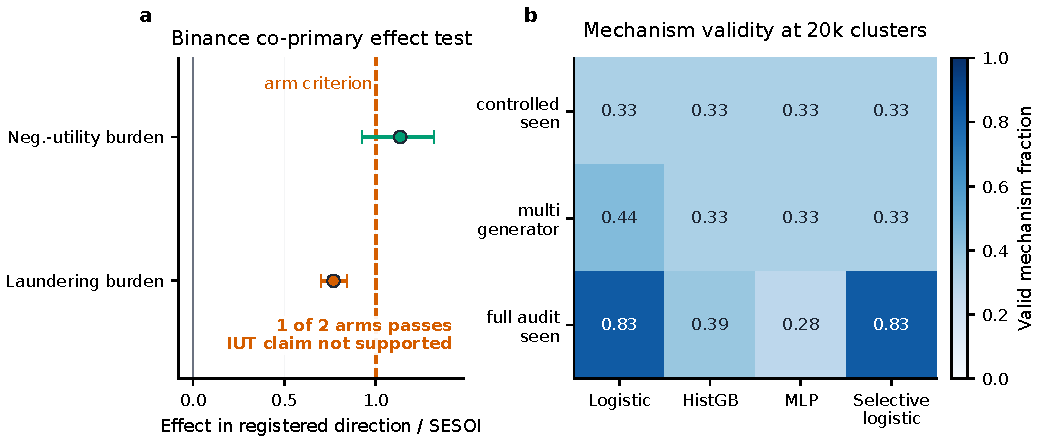
\includegraphics[width=\textwidth]{figures/fig_validity_gates.pdf}
  \Description{Two-panel validity-gate figure. The left panel shows two normalized co-primary effects from the powered Binance order-book test: negative-utility burden exceeds its registered effect threshold, while laundering burden remains below its threshold, so the intersection-union claim fails. The right panel shows valid-mechanism fractions at twenty thousand training clusters for three curricula and four learners.}
  \caption{\textbf{Validity gates preserve partial and undefined evidence.} Panel (a) divides registered Binance effects by their SESOIs; error bars are 95\% cluster-bootstrap intervals and the dashed line is the arm criterion. Planning power uses frozen v0.2 variance. Only one arm passes. Panel (b) reports the fraction of six mechanisms with coverage LCB at least 0.05 at 20,000 clusters; no cell reaches one.}
  \label{fig:validity_gates}
\end{figure*}

\begin{table}[t]
  \caption{Mechanism coverage invalidates most training endpoints (validation only). D0 is outside the data-utility Holm family; the role-neutral control is a negative control.}
  \label{tab:training_validity_supp}
  \centering
  \benchmarktableformat
  % Generated by finauth_audit/paper/generate_tables.py. Do not edit manually.
\begin{tabular}{lrp{0.39\linewidth}}
\toprule
Variant & Valid endpoints & Interpretation \\
\midrule
D0 & 5/5 & prediction diagnostic \\
D1 & 0/5 & authorization reference \\
D2 & 0/5 & authorization variant \\
D3 & 0/5 & authorization variant \\
D4 & 0/5 & authorization variant \\
D5 & 1/5 & authorization variant \\
D6 & 0/5 & authorization variant \\
D7 & 0/5 & authorization variant \\
D7 role-neutral & 0/5 & negative control; outside Holm \\
\bottomrule
\end{tabular}

\end{table}

\begin{table}[t]
  \caption{Holm-adjusted D2--D7 versus D1 validation contrasts. Delta NUAR is \textit{N/A} because no candidate/reference pair has valid endpoints in the same seed.}
  \label{tab:training_holm}
  \centering
  \benchmarktableformat
  % Generated by finauth_audit/paper/generate_tables.py. Do not edit manually.
\begin{tabular}{lrrrrl}
\toprule
Contrast & Delta NUAR & Valid pairs & Raw p & Holm p & Reject \\
\midrule
D2 vs D1 & \textit{N/A} & 0 & 1.000 & 1.000 & no \\
D3 vs D1 & \textit{N/A} & 0 & 1.000 & 1.000 & no \\
D4 vs D1 & \textit{N/A} & 0 & 1.000 & 1.000 & no \\
D5 vs D1 & \textit{N/A} & 0 & 1.000 & 1.000 & no \\
D6 vs D1 & \textit{N/A} & 0 & 1.000 & 1.000 & no \\
D7 vs D1 & \textit{N/A} & 0 & 1.000 & 1.000 & no \\
\bottomrule
\end{tabular}

\end{table}

The D7 role-neutral control masks role and lineage fields during training, calibration, and evaluation. It has 0/5 valid endpoints. Feature-group masking also shows that the fixed learner depends materially on role features: masking them raises D7 validation-unseen NUAR to 0.167 and ALR to 0.165. These are shortcut diagnostics, not causal feature attributions.

The prospective v0.3 robustness study uses Logistic Regression, histogram gradient boosting, MLP, and coverage-constrained selective Logistic; budgets of 400, 1,000, 5,000, and 20,000 independent clusters; controlled-seen, multi-generator, and full-audit-seen curricula; and three frozen seeds. At 20,000 clusters, full-audit Logistic and selective Logistic reach mean valid-mechanism fraction 0.833, but neither has all six mechanisms valid in any seed. Sequential-market validation remains below the fixed 0.05 coverage floor, so complete primary NUAR remains \textit{N/A}. This distinguishes partial endpoint recovery from a valid cross-mechanism comparison.

\section{Paper-Test Stability and Generator Sensitivity}
The paper split reproduces validation rankings, while the prospective mechanisms test whether that stability extends beyond one generator family.

\begin{table}[t]
  \caption{Validation-to-paper and cross-generator rank stability. Constant certification ranks remain \textit{N/A} and are not shown.}
  \label{tab:scale_stability}
  \centering
  \benchmarktableformat
  % Generated by finauth_audit/paper/generate_tables.py. Do not edit manually.
\begin{tabular}{p{0.48\linewidth}p{0.24\linewidth}r}
\toprule
Comparison & Rank & Spearman \\
\midrule
Validation vs paper test & raw FAR & 1.000 \\
Validation vs paper test & certification & 1.000 \\
Institutional vs Sequential & raw FAR & 0.994 \\
Institutional vs Utility IID & raw FAR & 0.738 \\
Sequential vs Utility IID & raw FAR & 0.683 \\
\bottomrule
\end{tabular}

\end{table}

Sequential and institutional generators have raw NUAR-rank Spearman 0.994; their correlations with utility IID are 0.683 and 0.738. Lowest-NUAR and highest-certification rules differ in two of three families. The controlled generators cannot establish a universal financial relationship; they supply interpretable, mechanistically distinct scenarios for auditing rule-by-generator interactions.

\section{Review Workload and Baseline Governance}
Review routing is not a free abstention channel. On validation, Lifecycle Checklist sends 43.5\% of controlled rows to review and exceeds a 40\% review-capacity scenario by 1,383 rows. Of those reviewed cases, 79.7\% would be harmful under direct execution, but only 1.9\% contain a safe positive opportunity. The paper-test review rate is 42.9\%. These are simulated workloads and normalized cost sensitivities, not measured staffing time or reviewer accuracy.

The baseline-governance audit reproduces the registered Lifecycle rule exactly, then evaluates frozen component removals and independently motivated compositions. Role + Confidence + Cost Gate and Lifecycle without the reduce route both achieve validation certification volume 0.60, above the registered Lifecycle value 0.30. Continuous conservative hypervolume instead ranks Hard Role Gate above Lifecycle. These results reject a Lifecycle-only winner narrative and support frontier reporting.

\section{Baseline Field Access}
Deployable rules may use candidate action, confidence, uncertainty, expected edge, cost and liquidity proxies, horizon, current source role, and legal lineage fields declared for their task. They may not use realized returns, post-cost utility, harm labels, oracle opportunity, laundering truth, tail loss, future decoys, or test outcomes. Oracle-positive opportunity and attack labels are evaluation-only. Public rationales, profiles, and user identities are not execution evidence.

The equal-information EPV Adapter uses the same legal fields as other baselines. It is included to test whether low NUAR transfers to provenance safety, not to establish or refute the companion method paper. The overlap audit snapshots the current AAAI source and checks seeds, exact data hashes, exact/perceptual figure hashes, headline claims, and shared 8/12-grams. The current audit reports zero conflicts across those gates; a fresh snapshot is required before submission.

\section{Negative Results and Change Policy}
FinAuth-Audit keeps development failures as audit evidence. The first controlled generator allowed non-opportunity noise to create unintended positive opportunities; a rule-independent correction repaired the density control. The first training endpoint averaged mechanisms before checking per-mechanism coverage and produced a misleading low-NUAR result; the registered endpoint now requires every mechanism to pass its coverage floor. Strict verification later found a cross-layer holdout leak in D4/D5/D7, after which both controlled and provenance holdout families were applied and the affected corpora rebuilt. No test outcome was opened during these changes.

After validation development, the existing test clusters were partitioned using event IDs only. A validation rehearsal reproduced registered outputs, the scientific surface was frozen in a content-addressed archive, and the paper-test evaluator was executed once. After inspection, generator distributions, attack definitions, seeds, feature manifests, certification thresholds, primary endpoints, and robustness profiles cannot change to obtain a preferred ranking. A correction requires a reproducible defect and a versioned record that preserves the original result. The 5,000-cluster community-hidden set remains unevaluated.

\section{Ethics and Responsible Use}
Controlled rows are synthetic authorization scenarios and can encode modeling assumptions or omit institutional constraints. Public rows contain event-market observations, not recommendations. The artifact must not be used to justify live trading, automated approval, or removal of human oversight. Users should report source provenance, decision-time legality, coverage, review load, and structural \textit{N/A}; publishing NUAR alone is insufficient. Any institutional extension should add expert review, privacy controls, jurisdiction-specific policy, and post-launch monitoring before operational use.

\FloatBarrier


\end{document}
